\chapter{Implementation}

\section{Linux Kernel Modification}
\begin{itemize}
  \item A patch implementing the SCTP send buffer advertisement was created for
    Linux kernel \texttt{v4.6-rc4}.
  \item The send buffer advertisement chunk type value was set to 150.
  \item To modify the frequency at which send buffer advertisement chunks are
    sent, a \texttt{sysctl} interface was created. The default value was set to
    5 seconds.
  \item A kernel timer was added corresponding to each SCTP association
    (within the \texttt{struct sctp\_association}).
  \item A state table was created for this chunk, specifying the states in which
    the send buffer advertisement chunk should be generated and sent.
\end{itemize}

\section{Test bed Implementation Details}
Two Raspberry Pis running Arch Linux were configured as routers by enabling
IP forwarding.
Laptops running the modified Linux kernel were used as end hosts.

\begin{figure}[h]
  \centering
  \small
  \begin{tikzpicture}[start chain=testbed going right]

    \node [on chain] {\vdots};

    \node [start branch=1 going above, on chain,
    label=below:PC\textsubscript{\(1\)},
    label=right:\texttt{\scriptsize 192.168.150.2}] (pc1)
    {
\includegraphics{imgs/pc.eps}};

    \node [start branch=2 going below, on chain,
    label=below:PC\textsubscript{\(x\)},
    label=right:\texttt{\scriptsize 192.168.150.x}] (pcn)
    {
\includegraphics{imgs/pc.eps}};

    \node [on chain, join=with pc1, join=with pcn,
    label=below:Switch\textsubscript{\(1\)}]
    {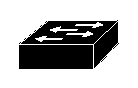
\includegraphics{imgs/switch.eps}};

    \node [on chain, join,
    label=below:RPi\textsubscript{\(1\)}] (rpi1)
    {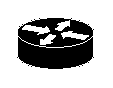
\includegraphics{imgs/router.eps}};

    \node [on chain, join,
    label=below:RPi\textsubscript{\(2\)}] (rpi2)
    {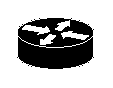
\includegraphics{imgs/router.eps}};

    \draw[-] (4.25, 0) -- (4.25, 0.5)
    node[above] {\scriptsize \texttt{192.168.150.1}};

    \draw[-] (8.45, 0) -- (8.45, 0.5)
    node[above] {\scriptsize \texttt{192.168.50.1}};

    \draw[-] (5.8, 0) -- (5.8, 1.5)
    node[above] {\scriptsize \texttt{192.168.100.2}};

    \draw[-] (6.85, 0) -- (6.85, -1.5)
    node[below] {\scriptsize \texttt{192.168.100.3}};

    \node [on chain, join,
    label=below:Switch\textsubscript{\(2\)}] (switch2)
    {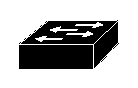
\includegraphics{imgs/switch.eps}};

    \node [on chain] {\vdots};

    \node [start branch=3 going above, on chain, join=with switch2,
    label=below:PC\textsubscript{\(x+1\)},
    label=left:\texttt{\scriptsize 192.168.50.2}]
    {
\includegraphics{imgs/pc.eps}};

    \node [start branch=4 going below, on chain, join=with switch2,
    label=below:PC\textsubscript{\(y\)},
    label=left:\texttt{\scriptsize 192.168.50.y}]
    {
\includegraphics{imgs/pc.eps}};

  \end{tikzpicture}
  \caption{Test bed implementation}
  \label{fig:testbed}
\end{figure}

The hosts in the test bed were allocated IP addresses as in figure
\ref{fig:testbed}.
From the figure, we observe that RPi\textsubscript{1}
would not be able to route packets with destination address in the
\texttt{192.168.50.0/24} subnet, and similarly RPi\textsubscript{2}
wouldn't be able to route packets directed to
\texttt{192.168.150.0/24} subnet. To enable end-to-end communication,
appropriate static routes were added to both the RPis.

The \texttt{tc} utility was used in the both the RPis to shape the
network flows in the bottleneck link. Larger bandwidth was
provided to flows with higher values of the percentage send buffer occupancy.

The Hierarchy Token Bucket classful queuing discipline was used to classify the
traffic into 11 classes, one of which is the default class used for non-SCTP
packets. The remaining 10 classes correspond to the send buffer occupancy
ranges of size 10.
\begin{figure}
  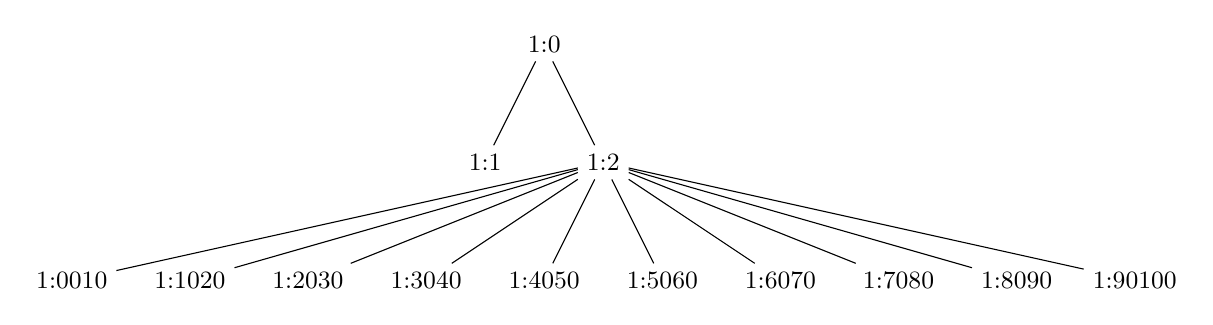
\begin{tikzpicture}
    \small
    \node{1:0}
    child { node {1:1} }
    child { node {1:2}
      child { node {1:0010} }
      child { node {1:1020} }
      child { node {1:2030} }
      child { node {1:3040} }
      child { node {1:4050} }
      child { node {1:5060} }
      child { node {1:6070} }
      child { node {1:7080} }
      child { node {1:8090} }
      child { node {1:90100} } };
  \end{tikzpicture}
  \caption{Hierarchy of classes}
\end{figure}
